\part{Working with R}
% ------------------------------------------------------------


%%%%%%%%%%%%%%%%%%%%%%%%%%%%%%%%%%%%%
% Section: Software Installation
\section{Installation}
\subsection{Software Installation}
%%%%%%%%%%%%%%%%%%%%%%%%%%%%%%%%%%%%%

\begin{frame}
  \frametitle{Installing R and RStudio}
    \begin{columns}
      \column{0.65\textwidth}
        \begin{enumerate}
           \item[R:] Go to \small \url{http://cran.r-project.org/}, select your operating system and download the latest version: 3.2.3 (Release 2015/12/10).
           \item[RStudio:] Go to \small \url{https://www.rstudio.com/products/rstudio/download/}, select your operating system and download the installer (if available).
        \end{enumerate}
%
      \column{0.35\textwidth}
       \begin{center}
         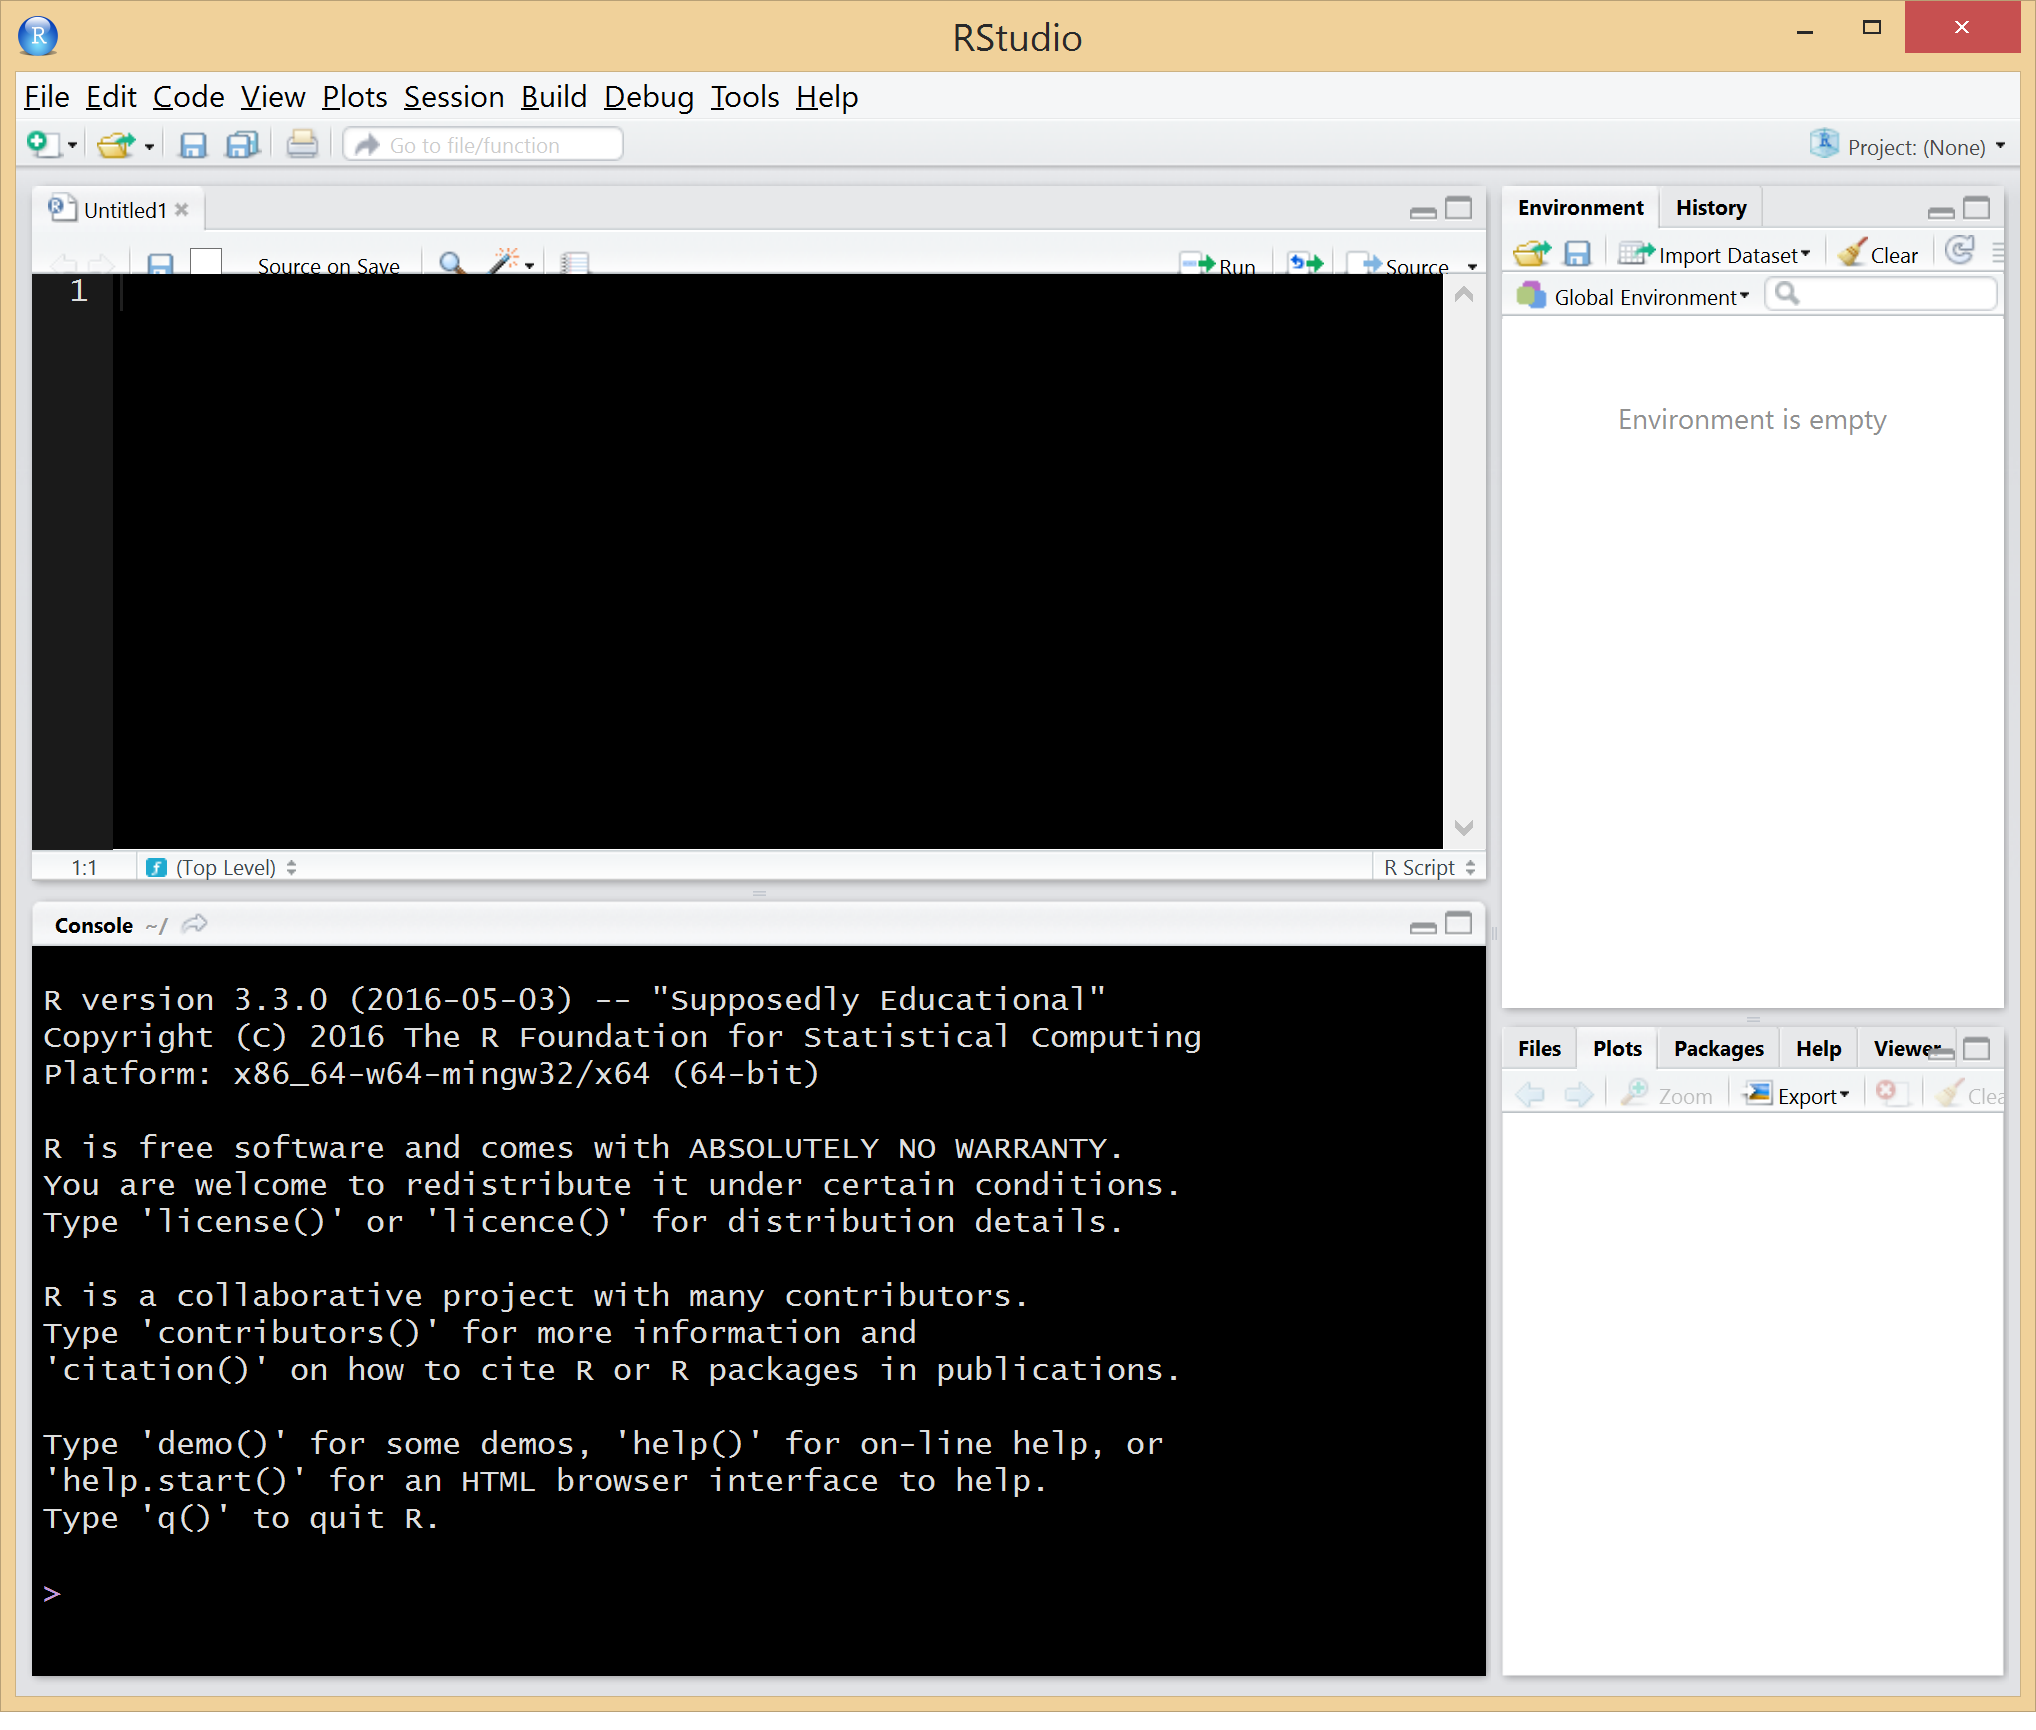
\includegraphics[width=1\textwidth]{images/Rwindow.png}
        \end{center}
      \end{columns}
\end{frame}

%%%%%%%%%%%%%%%%%%%%%%%%%%%%%%%%%%%%%
% Subsection: package installation
\subsection{Package Installation}
%%%%%%%%%%%%%%%%%%%%%%%%%%%%%%%%%%%%%

\begin{frame}[fragile]
  \frametitle{Package Installation}

  To install a package in R, use \ttfamily install.packages()\normalfont:
  \begin{lstlisting}
install.packages("lattice")
install.packages("ggplot2")
# OR
install.packages( c("lattice", "ggplot2") )
  \end{lstlisting}

\end{frame}

%---
%%%%%%%%%%%%%%%%%%%%%%%
\subsection{Saving Plots as a PDF} 
%%%%%%%%%%%%%%%%%%%%%%%
\begin{frame}[fragile]
\frametitle{Saving Plots as a PDF}
  \framesubtitle{For Static Plots}

  \itshape Note: \normalfont The files will be saved in the folder specified with \ttfamily setwd(). \normalfont
  To save a static plot in \ttfamily R \normalfont as a PDF, use function \ttfamily pdf(): \normalfont

  \begin{lstlisting}
# To save the image to the desktop:
setwd("~/Desktop")
pdf("filename.pdf")
wireframe(volcano, col.regions = terrain.colors(100), asp = 1, color.key=TRUE, drape=TRUE, scales = list(arrows = FALSE))
dev.off()
  \end{lstlisting}

\end{frame}

\begin{frame}[fragile]
  \frametitle{Saving Plots as a PDF}
  \framesubtitle{For Dynamic Plots}

  \itshape Note: \normalfont The files will be saved in the folder specified with \ttfamily setwd(). \normalfont
  To save a dynamic plot in \ttfamily R \normalfont as a PDF, use function \ttfamily rgl.snapshot(): \normalfont

  \begin{lstlisting}
# To save the image to the desktop:
setwd("~/Desktop")
# Step 1: Produce the 3D image:
plot3d(x=quakes$long, y=quakes$lat, z=quakes$depth, xlab="Longitude", ylab="Latitude", zlab="Depth")
# Step 2: Can rotate before taking a snapshot:
rgl.snapshot("quakes.png")
  \end{lstlisting}

\end{frame}

%%%%%%%%%%%%%%%%% 
\section[Error Messages]{Most Common Error Messages}
%%%%%%%%%%%%%%%%%%%%%%%%%%%%%%%%%%%%%

\begin{frame}
  \frametitle{Most Common Error Messages}

\end{frame}

%%%%%%%%%%%%%%%%%%%%%%%%%%%%%%%%%%%%%
% Section: R Help
\section[Help]{Getting R Help}
%%%%%%%%%%%%%%%%%%%%%%%%%%%%%%%%%%%%%

\begin{frame}[fragile]
\frametitle{R Help: Approach 1}

  \begin{columns}
  \column{0.4\textwidth}
  For help with any function in R, put a question mark before the function name to determine what arguments to use, examples and background information.

  \begin{lstlisting}
?plot
  \end{lstlisting}

  \column{0.6\textwidth}
    \begin{center}
    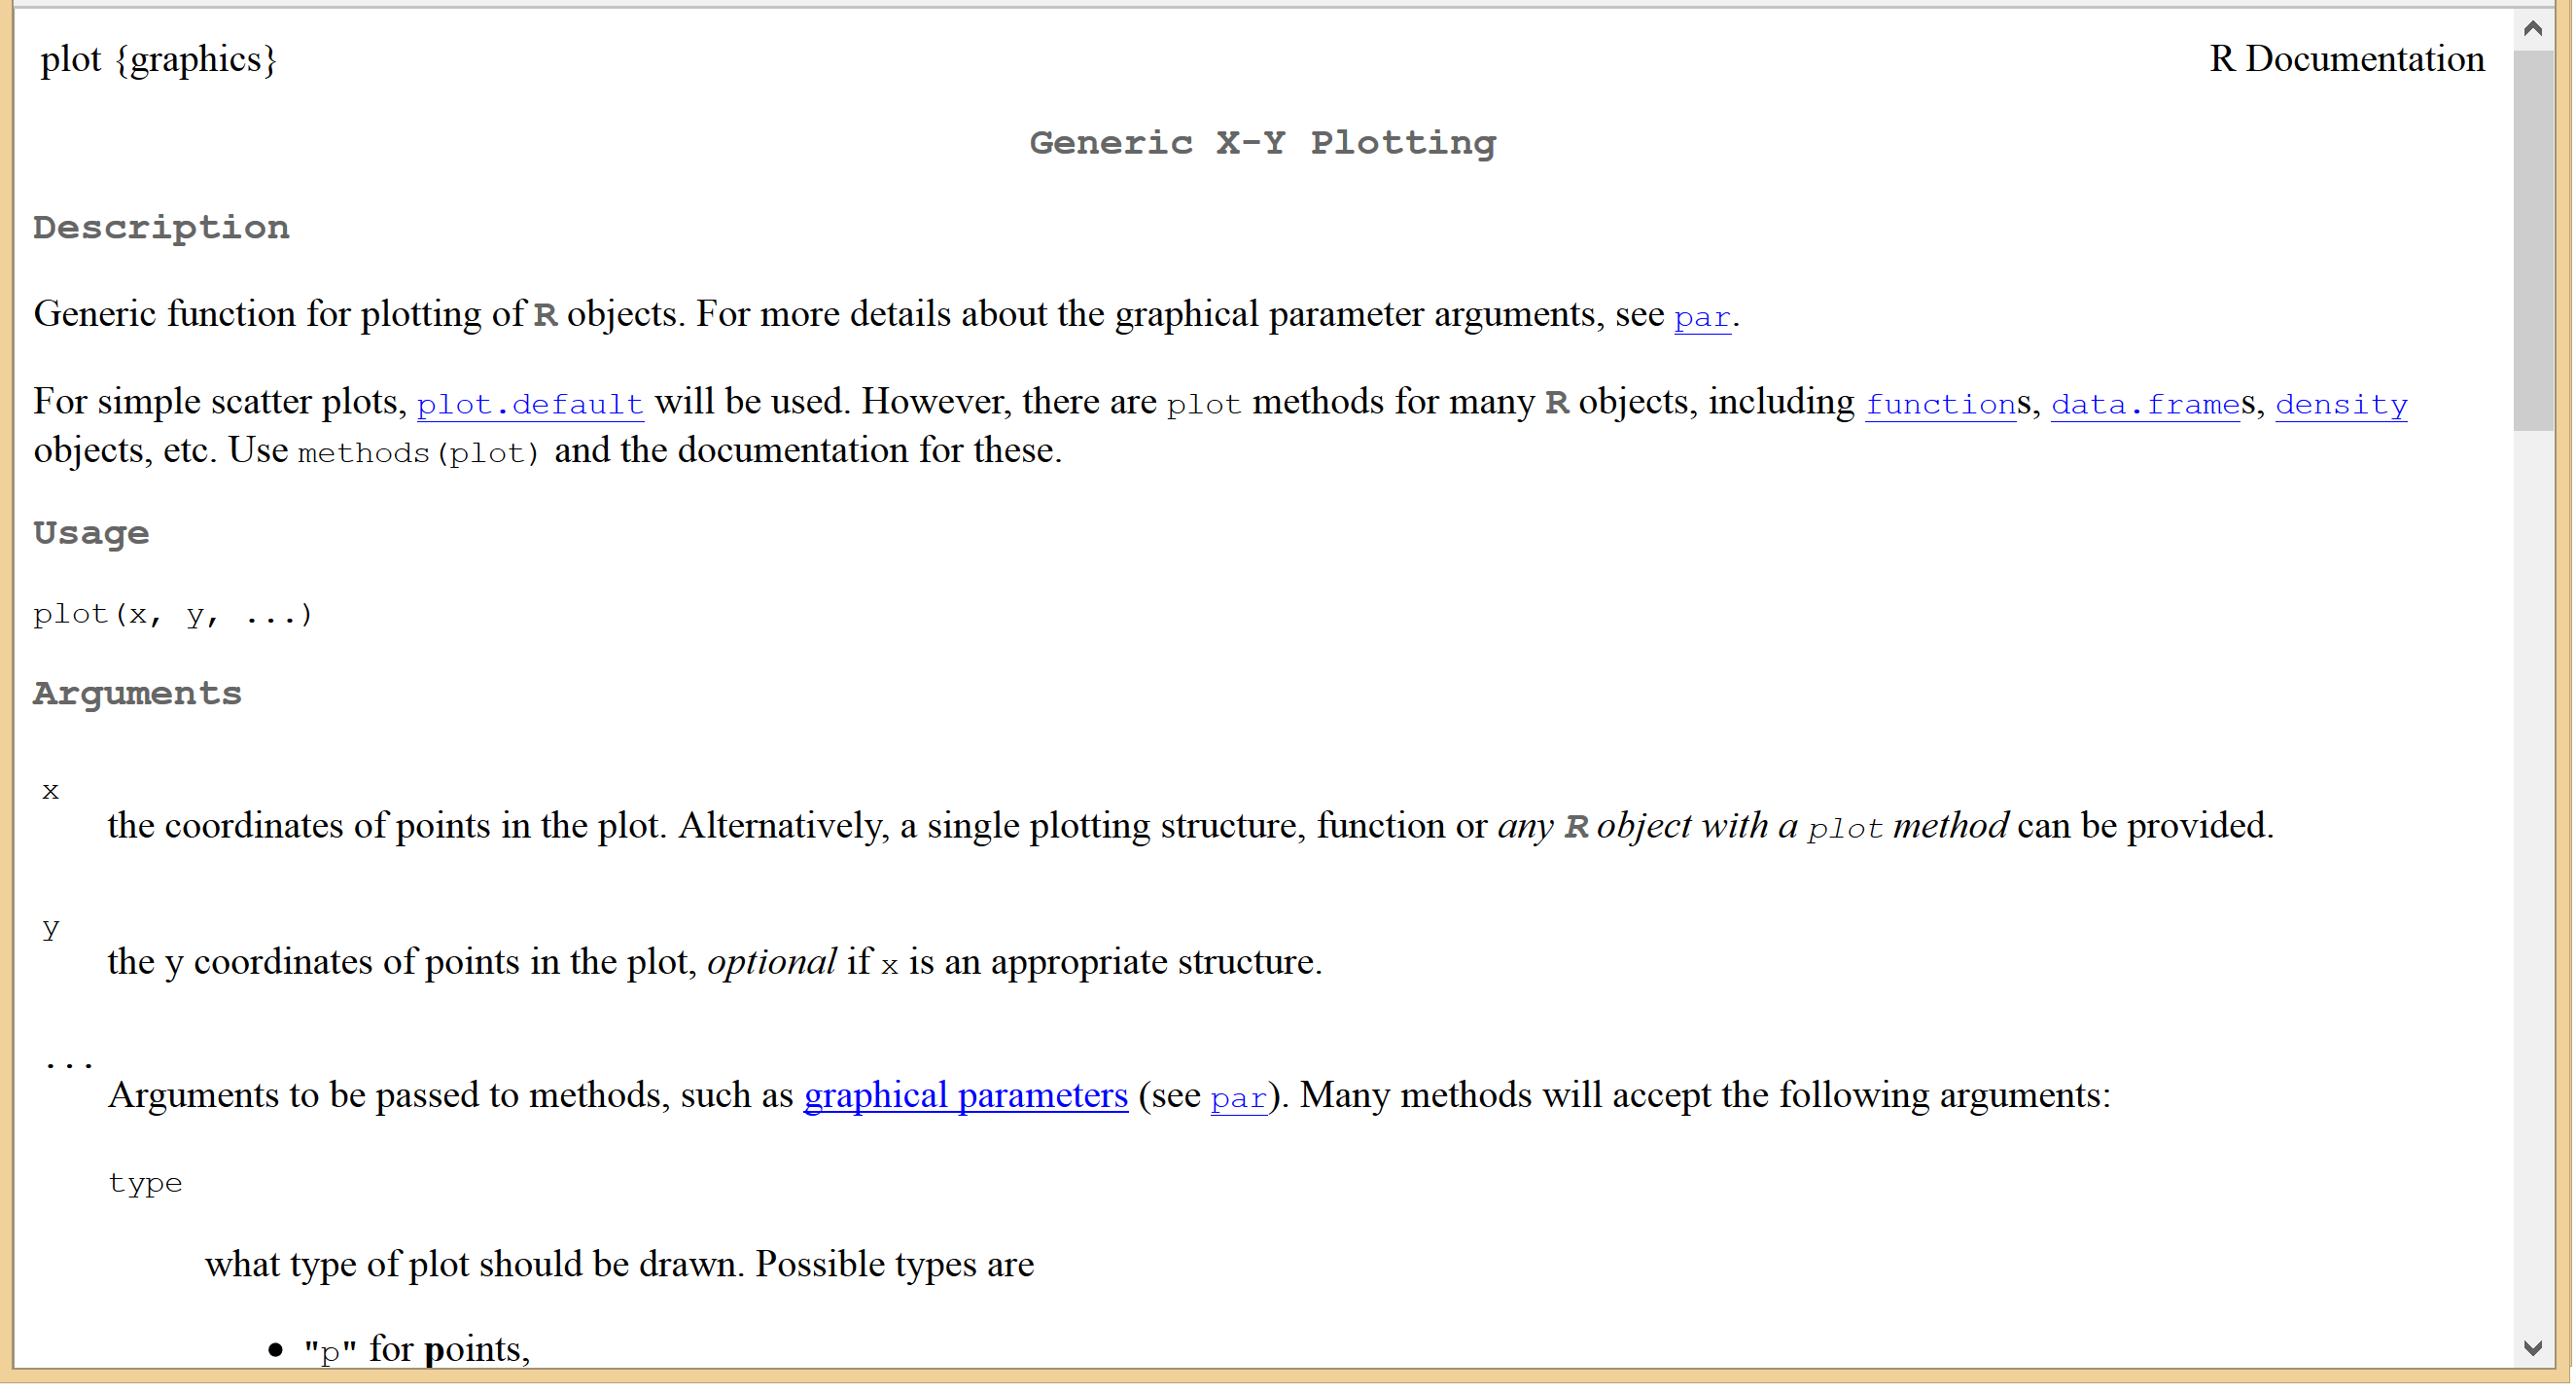
\includegraphics[width=1.1\textwidth]{images/Rhelp}
    \end{center}
  \end{columns}

\end{frame}
%%%---

\begin{frame}[fragile]
\frametitle{R Help: Approaches 2 and 3}

  \begin{columns}
  \column{0.6\textwidth}
  \begin{itemize}
    \item For help with any function in R, search answers on StackOverflow (SO).
    \item For help with any function in R, when all else fails, ask a question on StackOverflow.  Don't forget to follow the SO tips: \url{http://stackoverflow.com/help/how-to-ask}
  \end{itemize}

  \column{0.4\textwidth}
  \begin{center}
  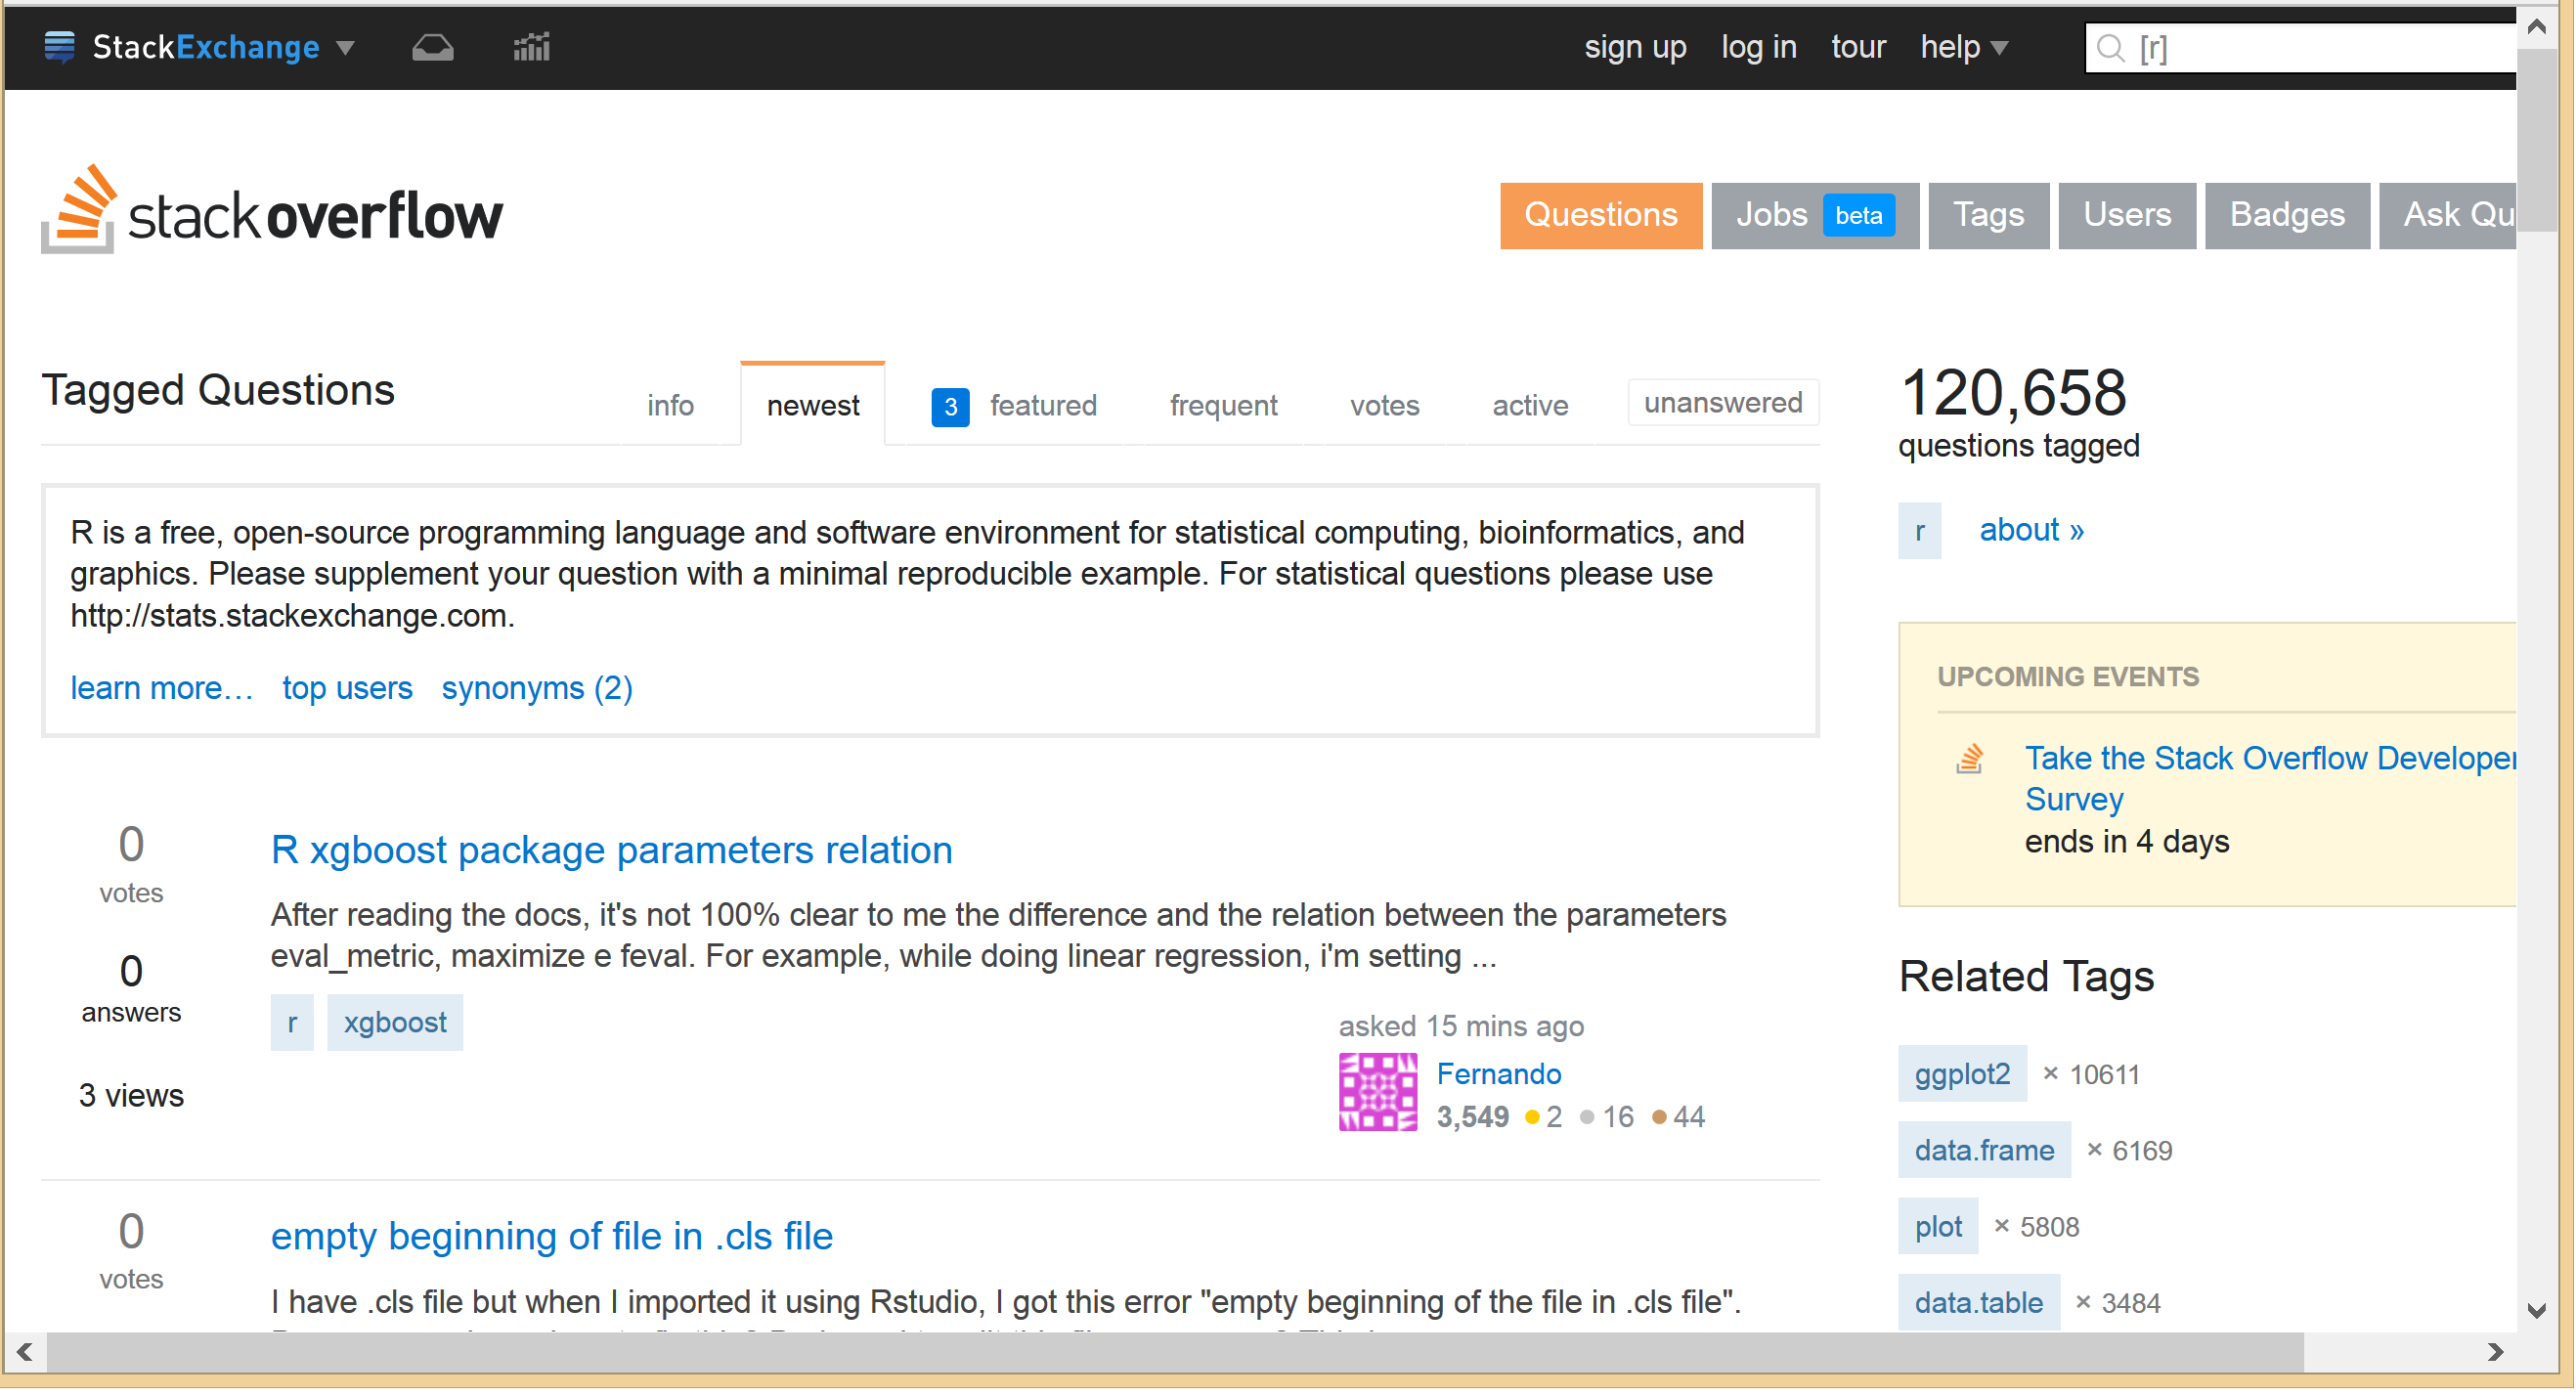
\includegraphics[width=0.95\textwidth]{images/SO}
  \end{center}
  \end{columns}

\end{frame}



%%%%%%%%%%%%%%%%%%%%%%%%%%%%%%%%%%%%%
%--- Online Resources
%%%%%%%%%%%%%%%%%%%%%%%%%%%%%%%%%%%%%
\section[Online Resources]{Online Resources for R}
\begin{frame}[fragile, allowframebreaks]
  \frametitle{Online Resources for R}
%\begin{description}[<+->] 
%\item[Download R:] http://cran.stat.ucla.edu/
%\item[Search Engine for R:] http://rseek.org
%\item[R Reference Card:] http://cran.r-project.org/doc/contrib/Short-refcard.pdf
%\item[UCLA Statistics Information Portal:] http://info.stat.ucla.edu/grad/
%\item[UCLA Statistical Consulting Center:] http://scc.stat.ucla.edu
%\end{description}

\begin{description}
	\item[Download R:] {\small \textit{\urlwofont{http://cran.stat.ucla.edu/}}}
  \item[Download RStudio:] {\small \textit{\urlwofont{https://www.rstudio.com/}}}  
	% \item[Search Engine for R:] {\small \textit{\urlwofont{http://rseek.org}}}
	\item[R Reference Card:] $\:$ \\
		{\small \textit{\urlwofont{http://cran.r-project.org/doc/contrib/Short-refcard.pdf}}}
	\item[R Graphics Gallery:] $\:$ \\
		 {\small \textit{\urlwofont{http://research.stowers-institute.org/efg/R/}}}
	\item[R Graph Gallery:]  {\small \textit{\urlwofont{http://addictedtor.free.fr/graphiques/}}}
	% \item[UCLA Statistics Information Portal:] \small{ \textit{\urlwofont{http://info.stat.ucla.edu/grad/}}}
	% \item[UCLA Statistical Consulting Center:] \small{ \textit{\urlwofont{http://scc.stat.ucla.edu}}}
  \item[] % Book on R graphics: http://book.flowingdata.com/
  \item[More R tutorials:] 
    \begin{itemize}
      \item[]
      \item[IK:] {\small \textit{\urlwofont{http://www.KukuyevaConsulting.com/tutorials}}}
      \item[UCLA IDRE:] {\small \textit{\urlwofont{http://www.ats.ucla.edu/stat/r/}}}
      \item[UCLA SCC:] {\small \textit{\urlwofont{http://scc.stat.ucla.edu/mini-courses/}}}
    \end{itemize}  
  \item[JSS:]
  \item[Stackoverflow:]
  \item[Blogs:]
\end{description}
\end{frame}


% http://adv-r.had.co.nz/ 
% http://www.statmethods.net/interface/packages.html package install
% List of packages https://cran.r-project.org/web/packages/
% Gallery: http://rgraphgallery.blogspot.com/search/label/barchart
% Steam charts: http://www.r-bloggers.com/data-mountains-and-streams-stacked-area-plots-in-r/

%%%%%%%%%%%%%%%%%%%%%%%%%%%%%%%%%%%%%
\section{References}
%%%%%%%%%%%%%%%%%%%%%%%%%%%%%%%%%%%%%

\begin{frame}
  \begin{itemize}
    \item[1.] \url{http://adv-r.had.co.nz/}
    \item[2.] \url{http://www.sixhat.net/how-to-plot-multpile-data-series-with-ggplot.html}
    \item[3.] \url{http://stackoverflow.com/questions/17584248/exact-axis-ticks-and-labels-in-r-lattice-xyplot}
    \item[4.] \url{https://rstudio-pubs-static.s3.amazonaws.com/3364_d1a578f521174152b46b19d0c83cbe7e.html}
    \item[5.] \url{www.jstatsoft.org/v25/c01/paper}
    \item[6.] \url{http://www.kdnuggets.com/2015/05/r-vs-python-data-science.html}
    \item[7.] \url{http://flowingdata.com/2014/02/05/where-people-run/}
    % \item[8.] \url{http://xkcd.com/688/}
    \item[8.] \url{https://www.facebook.com/notes/facebook-engineering/visualizing-friendships/469716398919}
  \end{itemize}
\end{frame}

%_________________________________ Part
%%%%%%%%%%%%%%%%%% Section: Exercise

%\frame{
%  \frametitle{Upcoming Mini-Course}
%	\framesubtitle{This Wednesday}
%$4:30$PM: Advanced Graphics with \ttfamily R \normalfont
%}

\frame{
  \frametitle{}
\begin{center}
Thank you.\\

Any questions?
\end{center}
}